%!TEX TS-program = xelatex

% Author: Amet Umerov (admin@amet13.name)
% https://github.com/Amet13/bachelor-diploma

\documentclass[a4paper,14pt]{extarticle} % 14й шрифт
%%% Преамбула %%%

\usepackage{fontspec} % XeTeX
\usepackage{xunicode} % Unicode для XeTeX
\usepackage{xltxtra}  % Верхние и нижние индексы
\usepackage{pdfpages} % Вставка PDF
\usepackage{array} % Работа с цами


\usepackage{listings} % Оформление исходного кода
\lstset{
    basicstyle=\small\ttfamily, % Размер и тип шрифта
    breaklines=true, % Перенос строк
    tabsize=2, % Размер табуляции
    literate={--}{{-{}-}}2 % Корректно отображать двойной дефис
}

% Шрифты, xelatex
\defaultfontfeatures{Ligatures=TeX}
\setmainfont{Times New Roman} % Нормоконтроллеры хотят именно его
\usepackage[english,russian]{babel}
%\newfontfamily\cyrillicfont{Times New Roman}
%\setsansfont{Liberation Sans} % Тут я его не использую, но если пригодится
%\setmonofont{FreeMono} % Моноширинный шрифт для оформления кода

% Русский язык
%\usepackage{polyglossia}
%\setdefaultlanguage{russian}


\usepackage{amssymb,amsfonts,amsmath} % Математика
\numberwithin{equation}{section} % Формула вида секция.номер

\usepackage{enumerate} % Тонкая настройка списков

\usepackage{indentfirst} % Красная строка после заголовка
\usepackage{float} % Расширенное управление плавающими объектами
\usepackage{multirow} % Сложные таблицы

% Пути к каталогам с изображениями
\usepackage{graphicx} % Вставка картинок и дополнений
\graphicspath{{images/}{images/userguide/}{images/testing/}{images/infrastructure/}{extra/}{extra/drafts/}}

% Формат подрисуночных записей
\usepackage{chngcntr}
\counterwithin{figure}{section}

% Гиперссылки
\usepackage{hyperref}
\hypersetup{
    colorlinks, urlcolor={black}, % Все ссылки черного цвета, кликабельные
    linkcolor={black}, citecolor={black}, filecolor={black},
    pdfauthor={Амет Умеров},
    pdftitle={Разработка виртуальной инфраструктуры для реализации облачных услуг}
}

% Оформление библиографии и подрисуночных записей через точку
\makeatletter
\renewcommand*{\@biblabel}[1]{\hfill#1.}
\renewcommand*\l@section{\@dottedtocline{1}{1em}{1em}}
\renewcommand{\thefigure}{\thesection.\arabic{figure}} % Формат рисунка секция.номер
\renewcommand{\thetable}{\arabic{table}} % Формат таблицы секция.номер
\def\redeflsection{\def\l@section{\@dottedtocline{1}{0em}{10em}}}
\makeatother

\renewcommand{\baselinestretch}{1.4} % Полуторный межстрочный интервал
\parindent 1.27cm % Абзацный отступ

\sloppy             % Избавляемся от переполнений
\hyphenpenalty=10000 % Частота переносов
\clubpenalty=10000  % Запрещаем разрыв страницы после первой строки абзаца
\widowpenalty=10000 % Запрещаем разрыв страницы после последней строки абзаца

% Отступы у страниц
\usepackage{geometry}
\geometry{left=3cm}
\geometry{right=1cm}
\geometry{top=2cm}
\geometry{bottom=2cm}

% Списки
\usepackage{enumitem}
%\setlist[enumerate,itemize]{leftmargin=12.7mm} % Отступы в списках
%\setlist[enumerate,itemize]{labelindent = 1.5cm, itemindent=0.55cm}
\setlist[itemize]{leftmargin=0mm, itemindent=1.8cm}
%\setlist[enumerate]{leftmargin=12.7mm} % Отступы в списках
\setlist[enumerate]{labelindent = 1.5cm, itemindent=0.55cm} % Отступы в списках
\makeatletter
    \AddEnumerateCounter{\asbuk}{\@asbuk}{м)}
\makeatother
\setlist{nolistsep} % Нет отступов между пунктами списка
\renewcommand{\labelitemi}{--} % Маркет списка --
%\renewcommand{\labelenumi}{\asbuk{enumi})} % Список второго уровня
%\renewcommand{\labelenumii}{\arabic{enumii})} % Список третьего уровня
%\renewcommand{\labelenumi}{\arabic{enumi}.\arabic{enumii}.}
\renewcommand{\labelenumi}{\arabic{enumi}}
%\renewcommand{\labelenumii}{\arabic{enumi})\arabic{enumii}.}
\renewcommand{\labelenumii}{\arabic{enumi}.\arabic{enumii}}
\renewcommand{\labelenumiii}{\arabic{enumi}.\arabic{enumii}.\arabic{enumiii}}

% Содержание
\usepackage{tocloft}
\renewcommand{\cfttoctitlefont}{\hspace{0.38\textwidth}\MakeTextUppercase} % СОДЕРЖАНИЕ
\renewcommand{\cftsecfont}{\hspace{0pt}}            % Имена секций в содержании не жирным шрифтом
\renewcommand\cftsecleader{\cftdotfill{\cftdotsep}} % Точки для секций в содержании
\renewcommand\cftsecpagefont{\mdseries}             % Номера страниц не жирные
\setcounter{tocdepth}{2}                            % Глубина оглавления, до subsubsection

% Нумерация страниц снизу посередине

\usepackage{fancyhdr}
\pagestyle{fancy}
\fancyhf{}
%\fancyhead[R]{\textrm{\thepage}}
%\fancyheadoffset{0mm}
%\fancyfootoffset{0mm}
%\setlength{\headheight}{17pt}

%\fancypagestyle{plain}{ 
%    \fancyhf{}
%    \rhead{\thepage}
%}
\fancyfoot[C]{\thepage}
\renewcommand{\headrulewidth}{0pt}
\renewcommand{\footrulewidth}{0pt}

% Формат подрисуночных надписей
\RequirePackage{caption}
\DeclareCaptionLabelSeparator{defffis}{ -- } % Разделитель
\captionsetup[figure]{justification=centering, labelsep=defffis, format=plain} % Подпись рисунка по центру
\captionsetup[table]{justification=raggedright, labelsep=defffis, format=plain, singlelinecheck=false} % Подпись таблицы слева
\addto\captionsrussian{\renewcommand{\figurename}{Рисунок}} % Имя фигуры

\raggedbottom
\captionsetup[figure]{belowskip=1.4pt,aboveskip=1.4pt}
\setlength{\intextsep}{1.4pt}

% Пользовательские функции
\newcommand{\addimg}[4]{ % Добавление одного рисунка
    \begin{figure}
        \centering
        \includegraphics[width=#2\linewidth]{#1}
        \caption{#3} \label{#4}
    \end{figure}
}
\newcommand{\addimghere}[4]{ % Добавить рисунок непосредственно в это место
    \begin{figure}[H]
    	\vspace{\baselineskip}
        \centering
        \includegraphics[width=#2\linewidth]{#1}
        \caption{#3} \label{#4}
    \end{figure}
}
\newcommand{\addtwoimghere}[5]{ % Вставка двух рисунков
    \begin{figure}[H]
        \centering
        \includegraphics[width=#2\linewidth]{#1}
        \hfill
        \includegraphics[width=#3\linewidth]{#2}
        \caption{#4} \label{#5}
    \end{figure}
}
\newcommand{\addimgapp}[2]{ % Это костыль для приложения Б
    \begin{figure}[H]
        \centering
        \includegraphics[width=1\linewidth]{#1}
        \caption*{#2}
    \end{figure}
}

% Заголовки секций в оглавлении в верхнем регистре
\usepackage{textcase}
\makeatletter
\let\oldcontentsline\contentsline
\def\contentsline#1#2{
	\expandafter\ifx\csname l@#1\endcsname\l@section
	\expandafter\@firstoftwo
	\else
	\expandafter\@secondoftwo
	\fi
	{\oldcontentsline{#1}{#2}}
	{\oldcontentsline{#1}{#2}}
}
\makeatother


% Оформление заголовков
\usepackage[compact,explicit]{titlesec}
\titleformat{\section}[block]{\vspace{0em}}{}{12.5mm}{\thesection\quad#1}%\vspace{1em}}
\titleformat{\subsection}[block]{\vspace{0em}}{}{12.5mm}{\thesubsection\quad#1}%\vspace{1em}}
\titleformat{\subsubsection}[block]{\vspace{0em}\normalsize}{}{12.5mm}{\thesubsubsection\quad#1}%\vspace{1em}}
\titleformat{\paragraph}[block]{\normalsize}{}{12.5mm}{#1}


\titlespacing{\section}{0pt}{0pt}{0pt}
\titlespacing{\subsection}{0pt}{0pt}{0pt}
\titlespacing{\subsubsection}{0pt}{0pt}{0pt}
\titlespacing{\paragraph}{0pt}{0pt}{0pt}



% Секции без номеров (введение, заключение...), вместо section*{}
\newcommand{\anonsection}[1]{
	\phantomsection % Корректный переход по ссылкам в содержании
	\paragraph{\centerline{{#1}}\vspace{1.5em}}
	\addcontentsline{toc}{section}{#1}
}

% Секции для приложений
\newcommand{\appsection}[1]{
	\phantomsection
	\paragraph{\centerline{{#1}}}
	\addcontentsline{toc}{section}{#1}
}

% Библиография: отступы и межстрочный интервал
\makeatletter
\renewenvironment{thebibliography}[1]
    {\section*{\refname}
        \list{\@biblabel{\@arabic\c@enumiv}}
           {\settowidth\labelwidth{\@biblabel{#1}}
            \leftmargin=0
            \labelsep
            \itemindent=1.7cm
            \@openbib@code
            \usecounter{enumiv}
            \let\p@enumiv\@empty
            \renewcommand\theenumiv{\@arabic\c@enumiv}
            %\renewcommand{\labelenumi}{\arabic{enumi}}
            %\renewcommand\theenumiv{\arabic{enumi}}
        }
        \setlength{\itemsep}{0pt}
    }
\makeatother

\makeatletter
\bibliographystyle{unsrt}
\renewcommand{\@biblabel}[1]{#1}
\makeatother

\AtBeginDocument{%
	\abovedisplayskip=10pt 
	\abovedisplayshortskip=10pt
	\belowdisplayskip=24pt
	\belowdisplayshortskip=24pt
}

\setcounter{page}{4} % Начало нумерации страниц
 % Подключаем преамбулу

%%% Начало документа
\begin{document}


%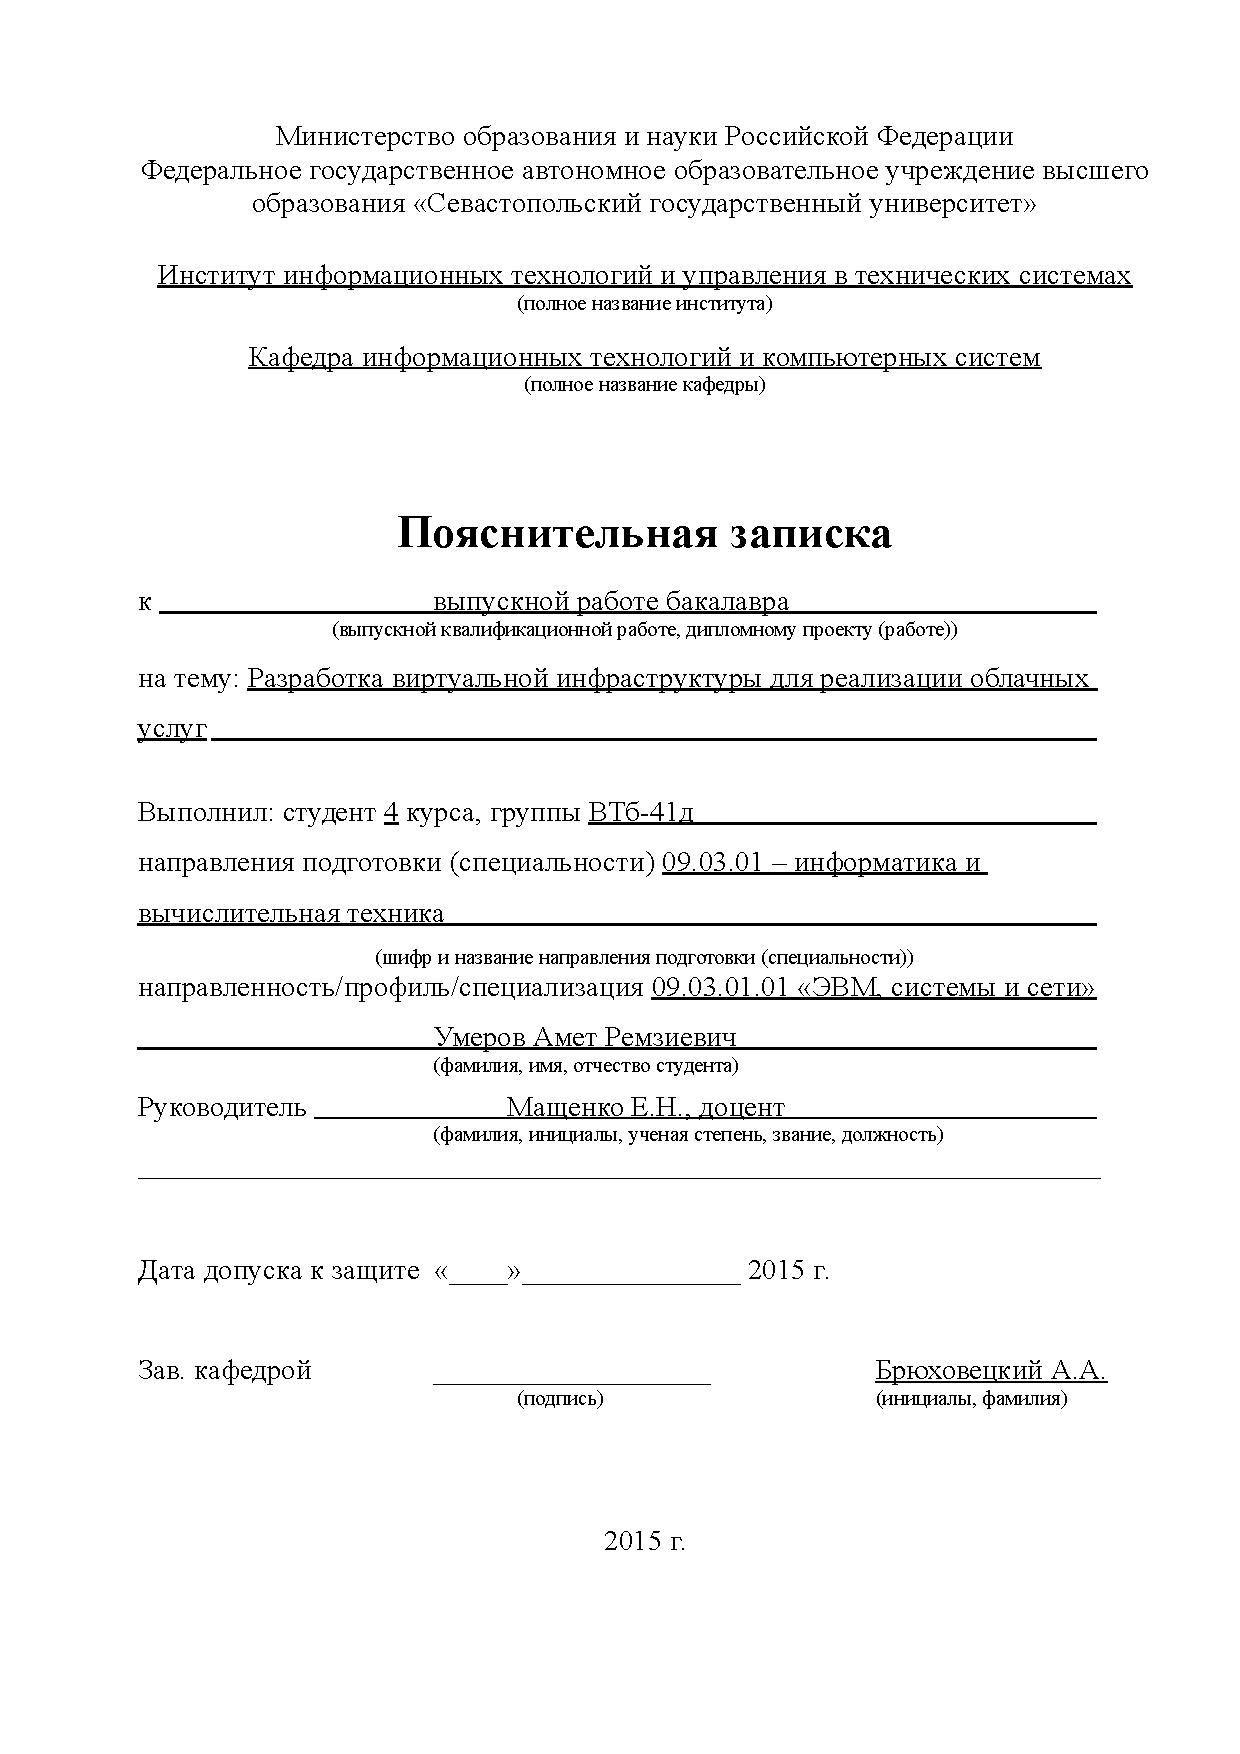
\includepdf{pz} % Пояснительная записка
%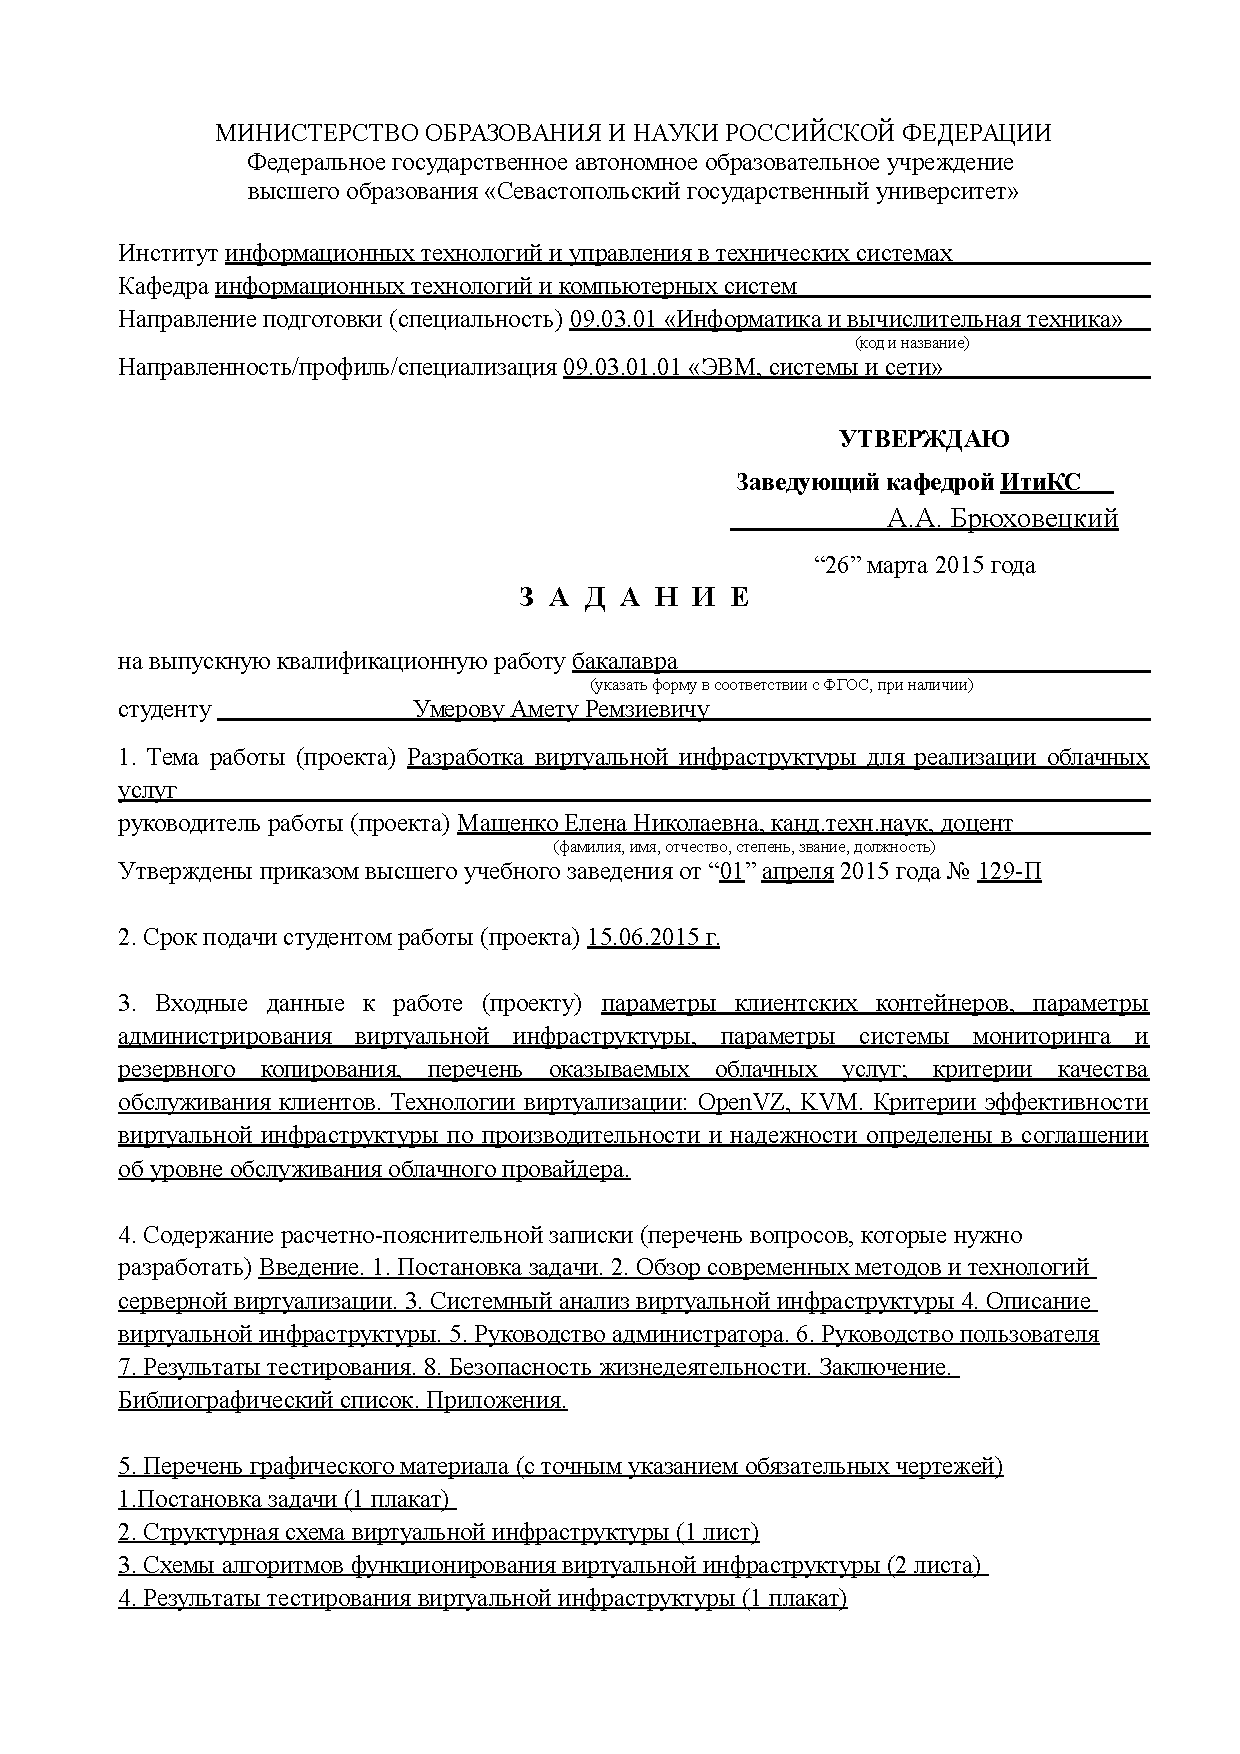
\includepdf[pages={1,2}]{task} % Задание на диплом печатается на одном листе с двух сторон
%помимо ПЗ и задания, в диплом также вкладывается отзыв руководителя и рецензия

\tableofcontents % Содержание 
\clearpage


%\anonsection{Введение}

Особый интерес к шагающим машинам появился в 1950-е годы после окончания второй мировой войны. Первой моделью «стопоходящей» машины была создана П.Л. Чебышевым. 
Способ передвижения с помощью ног, является наиболее распространенным в живой природе. 
Однако в технике он еще не получил заметного применения, прежде всего из-за сложности управления.
Основными преимуществами шагающих роботов -- является большая проходимость на пересеченной местности вплоть до возможности передвигаться прыжками и лазать по наклонным поверхностям по сравнению с колесными роботами \cite{urevich}. 

Применение шагающих роботов актуально при работе в опасных зонах, в том числе при устранении аварий техногенного характера и стихийных бедствий. 
В данных ситуациях необходимо исключить риск причинения вреда спасателям, а проходимости колесных роботов будет недостаточно.
Главными проблемами алгоритмов управления шагающими роботами являются:
\begin{itemize}
	\item сложность разработки алгоритма из-за большего числа решаемых подзадач;
	\item неустойчивость разработанного алгоритма к новым внешним условиям;
\end{itemize}

В данной работе будут рассмотрены основные подходы к созданию алгоритмов управления шагающими роботами, а также их сравнение. 
Цель сравнения выбрать подход для благодаря которому будут решены указанные проблемы. 
Для выбранного подхода будет проведен анализ и сравнения существующих решений и выбор наилучших.

\clearpage
 % Введение
\anonsection{Введение}


Несмотря на огромные достижения в области автоматизации, до сих пор существуют сферы человеческой деятельности, автоматизация которых либо крайне неэффективна, либо вообще не представляется возможной, когда, казалось бы, весьма несложные операции (с которыми легко справляется любой малоквалифицированный персонал) вообще не поддаются автоматизации. Заполнить многие из таких «свободных от автоматизации ниш» могли бы высокоадаптивные и автономные мобильные роботы (МР). 


«Интеллектуализация» МР является важнейшим направлением развития МР. Под этим термином здесь понимается повышение уровня адаптивности МР к сложным быстроизменяющимся внешним условиям или повышение степени независимости (автономности) процесса функционирования МР от человека-оператора. С увеличением степени автономности МР упрощается процесс управления роботом, уменьшается отрицательное влияние человеческого фактора, возрастает общая эффективность от применения МР.


Основные трудности при этом состоят в создании алгоритмического обеспечения, позволяющего автоматически управлять движением роботов, используя информацию о его положении относительно инерциальной системы координат и препятствий местности.


Однако при наличии большого числа публикаций, в которых используются как классические, так и современные подходы к синтезу алгоритмов обработки информации и управления, задача остается не решенной в полной мере. Это связано с излишней идеализированностью ее постановки, не учитывающей принципиальную невозможность знания точной математической модели робота, из-за отсутствия учета возможностей и характеристик реальных датчиков и желания авторов решить плохо формализуемую проблему управления при наличии большого количества разнородной информации на основе одного, порой достаточно сложного алгоритма.


Учитывая успехи алгоритмов глубокого обучения в различных плохо формализуемых задачах, было решено проанализировать и сравнить качество синтеза алгоритмов управления автономными роботами  на основе нейронных сетей с классическими не нейросетевыми алгоритмами.


Таким образом, актуальность задачи создания алгоритмов системы управления мобильных роботов на основе нейронных сетей, с одной стороны, определяется востребованностью автономных мобильных роботов, с другой - отсутствием эффективных алгоритмов, способных автономно решать плохо формализуемую задачу управления автономным роботом в различных средах.


\clearpage
 % Введение

\section{Анализ подходов к созданию автономных робототехнических систем} \label{literature}

Для синтеза алгоритмов управления автономными роботами наиболее актуальными являются следующие подходы:
\begin{itemize}
	\item эволюционные алгоритмы;
	\item подход на основе нечеткой логики;
	\item формальный подход;
	\item обучение с подкреплением.

\end{itemize}

Далее упомянутые подходы будут рассмотрены подробнее с целью выявить наилучший для решения задачи адаптивного управления шагающим роботом. 
%Далее упомянутые подходы будут рассмотрены подробнее с целью выявить наилучший для решения задачи управления автономным мобильным роботом. 
Выбор будет происходить по следующим критериям:
\begin{itemize}
	\item сложность формализации;
	\item возможность работать в неизвестной среде;
	\item сложность имплементирования;
	\item требовательность к вычислительным ресурсам.
\end{itemize}

Простота формализации является главным критерием, так как главной задачей является упрощение существующих методов создания алгоритмов управления. 
Работа в заранее неизвестной среде обусловлена адаптивностью алгоритма. 
Критерий сложности имплементирования определяет степень сложности воспроизведения алгоритма для новых начальных условий и конфигураций робота. 
Критерий требовательности к вычислительным ресурсам напрямую влияет на стоимость применения выбранного подхода.


\subsection{Эволюционные алгоритмы}

Эволюционные алгоритмы (ЭА) – это алгоритмы, созданные в качестве методов решения оптимизационных задач и основанные на принципах естественного отбора. 
ЭА моделируют базовые положения в теории биологической эволюции -- процессы отбора (селекции), мутации и воспроизводства. 
Множество агентов, называемое популяцией, эволюционирует согласно правилам отбора в соответствии с целевой функцией. Таким образом, каждому агенту (индивидууму) популяции назначается значение его приспособленности (значение фитнесс-функции, являющейся частным случаем целевой функции) в окружающей среде. 
Размножение и мутация позволяют изменяться агентам и приспособляться к среде \cite{evolution}.

В робототехнике применение ЭА позволяет выполнять различные практические задачи, в частности задачи обследования местности и маневрирования между препятствиями. 
Для агентов (роботов) описывается алгоритм, позволяющий им обмениваться генетической информацией с целью адаптации к решению конкретной задачи. 
В качестве генетической информации выступают различные стратегии управления приводами и системами робота на основе конкретных входных значений с датчиков. 
Такие стратегии могут задаваться изначально как случайно, так и согласно какой-либо эвристике. 
Цель – научить робота взаимодействовать с неизвестной средой. 

Преимущества эволюционного подхода:
\begin{itemize}
	\item возможность использования в задачах, сложно или полностью не поддающихся анализу и формализации;
	\item устойчивость в задачах с изменяющейся и/или частично неизвестной средой;
	\item существование большого количества как естественных, так и созданных человеком вариаций генетических операций.
\end{itemize}

Недостатки эволюционного подхода:
\begin{itemize}
	\item оценка функции приспособленности (фитнесс-функции) для сложных проблем (задачи высокой размерности) требует больших вычислительных мощностей, что часто является фактором, ограничивающим использование алгоритмов искусственной эволюции;
	\item кодирование генетической информации (иногда называется геномом или хромосомами) представляет собой также сложный процесс, пусть и менее сложный, чем формализация всей задачи;
	\item симуляция на настоящих роботах требует большого объёма ресурсов, поэтому обычно синтез алгоритма производят в компьютерных симуляциях, а затем полученные алгоритмы встраиваются в настоящие роботы. Однако процесс создания самой симуляции также является трудоёмким.
\end{itemize}


\subsection{Алгоритмы на основе нечёткой логики}

Нечёткая логика -- это раздел математики, являющийся обобщением логики и теории множеств, главным объектом исследования является нечеткое множество. 
В 1965 году Лотфи Заде расширил классическое понятие множества, допустив, что функция принадлежности принимает не только значения 0 и 1, а интервал от 0 до 1 \cite{fuzzy}. 
Традиционный логический блок компьютера может давать определенный ответ -- правда или ложь, что эквивалентно человеческим да или нет. 
Подход нечеткой логики позволяет давать более гибкие ответы, определяя аналоги человеческим: «возможно да», «не могу сказать», «возможно нет» и так далее. 

Архитектура системы нечеткой логики состоит из четырёх основных частей:
\begin{itemize}
	\item фузификатор (от английского fuzzy -- нечеткий); 
	\item база знаний;
	\item блок обработки; 
	\item дефузификатор.
\end{itemize}

Фузификатор -- модуль трансформирующий входной сигнал в элемент нечеткого множества. 
Входом может быть сигнал измеренный сенсорами например температура или скорость. 
Обычно трансформированный сигнал делится на пять диапазонов:
\begin{itemize}
	\item LP -- вход большой положительный;
	\item MP -- вход средний положительный;
	\item S -- вход малый;
	\item MN -- вход средний отрицательный;
	\item LN -- вход большой отрицательный.
\end{itemize}

Функция, которая  определяет отображение из пространства входов в интервал от 0 до 1, называется функцией принадлежности. 
В основном они используют 3 типа сигналов:
\begin{itemize}
	\item испульсный;
	\item гауссовый;
	\item треугольный или трапецеидальный.
\end{itemize}

Пример треугольного сигнала для перевода напряжения в интервал от 0 до 1 приведен на рисунке \ref{fuzzy}.
\addimghere{fuzzy}{1}{Пример треугольного сигнала}{fuzzy} 

База знаний  -- база созданная экспертами в той области, которой реализуется система. 
В ней содержится набор условных правил.

Блок обработки -- модуль обрабатывающий входное значения, используя правила из базы знаний.

Дефузификатор -- трансформирует обработанный вход из нечеткого логики в классическую.

На рисунке \ref{fuzzysch} показана схема работы данной системы.
\addimghere{fuzzysch}{0.5}{Схема работы системы, использующей нечеткую логику.}{fuzzysch} 

Нечеткую логику используют в робототехнике для создания систем управления, систем стабилизации, экспертных систем и в случаях когда необходимо сделать систему реагирующую как человек или для работы совместно с человеком \cite{fuzzy1}, \cite{fuzzy2}, \cite{fuzzy3}.

Достоинства подхода, использующего нечеткую логику:
\begin{itemize}
	\item подход устойчив к шуму входного сигнала;
	\item архитектура подхода понятна и проста в использовании;
	\item гибкость внесения изменений, достаточно изменить правило в базе знаний.
\end{itemize}

Недостатки подхода, использующего нечеткую логику:
\begin{itemize}
	\item нет систематического подхода для построения архитектуры под каждую задачу;
	\item подход остается понятным, только когда архитектура не сложна;
	\item подход не дает высокой точности.
\end{itemize}


\subsection{Формальный подход}
Формализация – представление в виде формальной системы какой-либо содержательной информации, представленной на естественном языке, путём изъятия логических свойств элементов естественного языка, существенных отношений между этими элементами, а также определение принципов  логической дедукции и критериев различия правильных способов рассуждения от неправильных.

%Исправь себе на адаптивный (только, желательно, в копии этого файла. Так же, как и с введением)
Задача синтеза алгоритма управления автономным роботом также требует формализации задачи, если она решается не методами искусственного интеллекта (ИИ). 
В задаче управления автономным мобильным роботом формализация заключается в составлении перечня всевозможных ситуаций, в которых может оказаться робот, и описание действий (и их порядка), которые необходимо в таких ситуациях предпринимать. 

Преимущества:
\begin{itemize}
	\item полная интерпретируемость алгоритма, т.е. возможность объяснить действия робота в любой ситуации;
	\item возможность оптимизации алгоритма управления.
\end{itemize}

Недостатки:
\begin{itemize}
	\item требование значительных человеческих и вычислительных ресурсов для анализа и формализации задачи, 
а также для составления и оптимизации алгоритма (зачастую уникального, т.е. для которого сложно найти примеры имплементации).
\end{itemize}


\subsection{Обучение с подкреплением}

Обучение с подкреплением -- это класс методов машинного обучения, при котором происходит обучение агента (робота), который не имеет сведений о среде, но имеет возможность производить какие-либо действия в ней. 
Действия агента переводят среду в новое состояние и агент получает от среды некоторое вознаграждение или наказание в соответствии с функцией подкрепления. 
Функция подкрепления определяет цель в процессе обучения с подкреплением и является по сути соответствием между состояниями среды и числом, подкреплением, показывающим желательность, ценность состояния. В качестве функции подкрепления может быть, например, расстояние от робота до определённой точки пространства; высота верхней точки шагающего робота (косвенно сообщающая о том, что робот не упал); уровень заряда батареи бортового аккумулятора.
В данном классе методов большое внимание уделяется поощрению/наказанию не только текущих действий, которые непосредственно привели к положительному/отрицательному подкреплению, но и тех действий, которые предшествовали текущим.
Поэтому в качестве целевой функции выступает сумма подкреплений на определённом промежутке пространства, например, суммарное подкрепление за прохождение определённой траектории.
В то время как функция подкрепления определяет прямую, характерную желательность состояния среды, целевая функция обнаруживает долгосрочную желательность состояний после принятия во внимание состояний, которые последуют за текущим, и подкреплений, соответствующих этим состояниям. 
Например, состояние может повлечь низкое непосредственное подкрепление, но при этом сильно положительно повлиять на суммарную оценку, потому как за ним регулярно следуют другие состояние, которые приносят высокие подкрепления. 
Единственная цель агента состоит в максимизации итогового подкрепления (целевой функции), которое тот получает в процессе длительной работы \cite{reinf_lern}.  

В робототехнике обучение с подкреплением активно применяется в задаче передвижения мобильного робота по лабиринту \cite{reinf_lern1} и в задаче управления манипулятором \cite{reinf_lern2}. 
Также существуют попытки обучать агента выполнять задачи разного плана при помощи одного алгоритма\cite{reinf_lern3}.

Преимущества обучения с подкреплением:
\begin{itemize}
	\item обучившаяся нейросеть позволяет решать общую задачу;
	\item для обучения нейросети требуется меньше вычислительных мощностей, чем в эволюционных методах;
	\item достаточно одного агента для обучения.	
\end{itemize}

Недостатки обучения с подкреплением:
\begin{itemize}
	\item требования к вычислительным ресурсам в случаях многоразмерных задач;
	\item в процессе обучения не всегда находится оптимальная стратегия для получения максимальной долгосрочной награды.
\end{itemize}


\subsection{Вывод по главе}

В данной главе были рассмотрены наиболее актуальные подходы для решения задачи синтеза алгоритма управления -- подход на основе нечеткой логики, эволюционный подход, подход на основе обучения с подкреплением, экспертный подход. 
Рассмотренные алгоритмы были сравнены между собой по критериям -- степень формализации, обобщающая способность, трудозатраты и требовательность к вычислительным ресурсам. 
Результаты сравнения представлены в \mbox{таблице \ref{table:ApDifference}.}

\begin{table}[H]
	\caption{Сравнение подходов к созданию систем управления}\label{table:ApDifference}
	\begin{tabular}{|m{3,8cm}|m{1,9cm}|m{2,7cm}|m{3,2cm}|m{3,2cm}|}
		\hline Критерий & Нечеткая логика & Формальный подход & Эволюционные алгоритмы &  Обучение с подкреплением \\
		\hline Сложность формализации  & Высокая & Высокая & Средняя & Малая  \\
		\hline Обобщающая способность & Нет & Нет & Да & Да \\
		\hline Трудозатраты  & Средне & Много & Средне & Мало \\
		\hline Требовательность к вычислительным ресурсам  & Мало & Мало & Много & Средне \\
		\hline 
	\end{tabular}
\end{table}

Степень формализации -- основной критерий, он показывает количество начальной информации необходимо знать об агенте и как полно необходимо описать кинематику и динамику агента. 
В методах эволюционном подходе и обучении с подкреплением происходит абстрагирование от физических характеристик агентов, благодаря этому трудозатраты на создание алгоритмов управления для сложных систем сокращаются. 
Также, из-за того, что в этих методах не используется описание конкретной задачи, а только функция содержащая общие аспекты работы алгоритма, то и сам алгоритм имеет большую обобщающую способность.

Для работы эволюционных методов необходима симуляция множества агентов, что сильно увеличивает требования к вычислительным ресурсам. 
Описание целевой функции в эволюционных методах и в обучении с подкреплением - относительно простая задача. Однако кодирование генома агента в эволюционных алгоритмах - несравненно больший труд.

В связи с вышесказанным, лучшим из рассмотренных методов по выбранным критериям является методы, использующие обучение с подкреплением.

\clearpage

 % Анализ подходов к созданию автономных робототехнических систем

\section{Анализ методов обучения с подкреплением}
Для решения задачи синтеза алгоритма управления был выбран подход с использованием обучения с подкреплением.
Алгоритмы обучения с подкреплением делятся на две группы:
\begin{itemize}
	\item с аналоговым выходом;
	\item с дискретным выходом.
\end{itemize}

Данные группы алгоритмов решают разные задачи: первые используются в системах, где управляющий сигнал представлен диапазоном значений, например, управление напряжением двигателя. 
Вторая группа алгоритмов используется в системах, где управляющий сигнал представлен конечным набором действий. 

В этой главе будут рассмотрены 3 алгоритма с аналоговым выходом:
\begin{itemize}
	\item DDPG;
	\item PPO;
	\item TRPO.
\end{itemize}

А также 4 алгоритма с дискретным выходом:
\begin{itemize}
	\item CEM;
	\item DQN;
	\item DUEL DQN;
	\item SARSA.
\end{itemize}

Вышеупомянутые алгоритмы сравнены между собой по критериям следующим критериям:
\begin{itemize}
	\item скорость обучения;
	\item качество;
	\item стабильность;
	\item количество обучаемый параметров.
\end{itemize}

\subsection{CEM}

Метод перекрестной энтропии (CEM) --общий алгоритм для решения глобальной оптимизационной задачи. 
Данный метод позволяет обучить нейронную сеть для решения задачи обучения с подкреплением. 
Нейронная сеть является управляющим звеном, на нее поступают выходы агента, например показания датчиков, а выходом нейронной сети являются входы агента, то есть стратегия управления.

На практике стратегия представляется, как распределения вероятности над действиями. 
Данный подход очень похож с задачей классификации, выбор одного действия из набора: алгоритм пропускает через нейронную сеть наблюдение окружающей среды, забирает вероятностное распределение над действиями (стратегию) и генерирует случайную выборку из этого распределения. 
Это случайная выборка добавляет неопределенности агенту, что хорошо влияет на начало обучающего процесса. Чем дольше происходит процесс обучения, тем меньше становится неопределенность. 
После действия, агент получает награду и цикл повторяется \cite{CEM}.

В процессе обучения мы минимизируем разницу между начальной стратегией и оптимальной, найденной методом выборки по значимости \cite{CEM1}, в итеративном процессе. 
Разность между текущей и оптимальной стратегией определяет дивергенция Кульбака-Лейблера -- формула (\ref{ fraq1 }).

\begin{equation}\label{ fraq1 }
\displaystyle D_{\mathrm {KL} }(P\|Q)=\int _{X}p\,\log {\frac {p}{q}}\,{\rm {d}}\mu 
\end{equation}

Где p(x), q(x) -- функции плотности распределения, сравниваемых величин.

Достоинства данного метода:
\begin{itemize}
	\item хорошо работает в легких средах;
	\item робастный к изменению гиперпарамтеров.
\end{itemize}

Недостатки CEM:
\begin{itemize}
	\item низкая скорость обучения.
\end{itemize}

\subsection{DQN}

Deep Q – Network (DQN) – улучшение классического алгоритма обучения с подкреплением Q-learning за счёт использования нейронных сетей.

Q-learning (в русскоязычной литературе иногда употребляется Q-обучение) – алгоритм, согласно которому агент на основе получаемого от среды вознаграждения формирует функцию полезности Q, что впоследствии дает ему возможность уже не случайно выбирать стратегию поведения, а учитывать опыт предыдущего взаимодействия со средой. 
Одно из преимуществ Q-обучения -- то, что оно в состоянии сравнить ожидаемую полезность доступных действий, не формируя модели окружающей среды. 
Применяется для ситуаций, которые можно представить в виде Марковского процесса принятия решений (англ. Markov decision process (MDP)), то есть процесса, в котором вероятности переходов между состояниями не зависят от истории предыдущих переходов. 

Алгоритм Q-learning пытается получить значение функции Q в явном виде для всех возможных пар «состояние среды - действие», чтобы потом максимизировать ожидаемый результат, найдя оптимальную стратегию. 
Однако даже в самых простых задачах робототехники число состояний среды очень велико, а если его умножить на количество возможных действий, то получится таблица, обрабатывать которую на борту робота будет затруднительно. 
Поэтому в алгоритме DQN таблица Q заменена функцией, которую приближает свёрточная нейронная сеть. 
Помимо этого, у DQN есть ещё несколько усовершенствований по сравнению с классическим алгоритмом Q-learning. 
Во-первых, практика показывает, что обучаться непосредственно на состояниях, происходящих друг за другом, -- плохая идея, так как такие состояния слишком похожи друг на друга, сильно коррелируют, причём со временем их распределение, естественно, сдвигается в зависимости от действий (или, например, положения) робота, но остается локализованным. 
Это мешает эффективному обучению, ведь в обычной постановке задачи обучения предполагается, что тренировочные данные независимы, а распределение данных со временем не меняется. 
Поэтому по мере обучения DQN сначала накапливает некоторый опыт, сохраняя свои действия и их результаты на протяжении какого-то времени, а потом выбирает из этого опыта случайную выборку (mini-batch) отдельных примеров для обучения, взятых в случайном порядке. 
Во-вторых, важную роль для успеха сыграло то, что при обучении DQN сеть, которая отвечала за целевую функцию, была отделена от сети, которая собственно обучается. 
Сделано это по причине того, что на практике нейронные сети довольно быстро заходят в локальные экстремумы и начинают очень глубоко исследовать глобально не необходимые части пространства поиска, бесцельно тратя ресурсы и фактически не обучаясь. 
Избежать этого можно сделав так, чтобы сеть не сразу использовала обновленную версию в целевой функции, а обучалась достаточно долгое время по старым образцам, прежде чем использовать обновлённую целевую функцию. 
В-третьих, на практике обычно применяется архитектура, в которой возможное действие агента не подается на вход, а просто у сети столько выходов, сколько возможных действий, и, получая на входе состояние, сеть пытается предсказать результаты полезности, ценности каждого действия (после чего, естественно, выбирает максимальный). 
Это важное улучшение, потому что оно позволяет получить ответы для сразу всех действий за один проход по сети, что ускоряет происходящее в разы, а сеть от этого сильно сложнее не становится, ведь основная часть ее «логики» остается прежней и используется заново.

Преимущества:
\begin{itemize}
	\item простой относительно других алгоритмов глубокого обучения с подкреплением, в следствие чего обучается быстрее более сложных алгоритмов;
	\item благодаря усовершенствованиям справляется с проблемой локальных минимумов.
\end{itemize}

Недостатки:
\begin{itemize}
	\item не использует всю историю обучения;
	\item может ограничивать скорость обучения.
\end{itemize}


\subsection{DUEL DQN}
Duel DQN является улучшением алгоритма DQN за счёт разделения Q-сети на два канала, один из которых вычисляет оценку позиции V, которая является функцией только состояния среды, а другой -- зависящую от действия функцию преимущества (advantage function) A. 
На последнем этапе они просто складываются в прежнюю функцию Q. 
Таким образом, одна часть сети обучается оценивать позицию как таковую, а другая -- предсказывать, насколько полезны будут разные наши действия в этой позиции. 
Такое небольшое изменение в архитектуре сети приближает смысл оценки к естественному, что часто существенно улучшает результаты \cite{DUEL_DQN}.
Сравнение архитектур DQN и DUEL DQN показана на рисунке \ref{dueldqn}.

\addimghere{dueldqn}{0.6}{Сравнение архитектур DQN(сверху) и DUEL DQN(снизу).}{dueldqn} 

\subsection{SARSA}
\subsection{DDPG}
%ДОБАВЬ ПЛЕЗ ИСТОЧНИКИ. Те, что прямо тут - они общее вдохновление дали. Остальные по месту употребления%
[Николенко книга]
[https://medium.freecodecamp.org/an-introduction-to-policy-gradients-with-cartpole-and-doom-495b5ef2207f]
[https://towardsdatascience.com/introduction-to-various-reinforcement-learning-algorithms-i-q-learning-sarsa-dqn-ddpg-72a5e0cb6287]
[https://www.cs.ubc.ca/~gberseth/blog/demystifying-the-many-deep-reinforcement-learning-algorithms.html]

В алгоритмах Q-learning, DQN, Duel DQN и SARSA действия выбираются согласно максимальному Q-значению. В таких алгоритмах (они называются value-based, то есть основанных на значениях функции Q) стратегия представляет собой ни что иное, как выбор действия с максимальным значением Q. Проблема value-based подхода заключается в необходимости вычисления оценки награды для каждого возможного действия в каждом возможном состоянии. Особенно остро эта проблема встаёт, когда дело касается бесконечного пространства действий (обычно это физические задачи, например, классическая задача балансировки обратного маятника. Также это задачи управления вращением колёс, движением манипулятора). Например, DQN создавался для решения проблемы с достаточно высокоразмерным пространством состояний (пиксели на экране в играх Atari), но при этом очень малоразмерным дискретным пространством действий (до двух десятков комбинаций кнопок). Но задачи физического контроля имеют непрерывные и высокоразмерные пространства действий. DQN не может быть непосредственно применён к непрерывным пространствам даже при грубой дискретизации пространства действий, так как размер выходного слоя нейронной сети Q-network растёт экспоненциально с ростом степеней свободы агента.

В алгоритмах градиентного спуска по стратегиям (policy gradient (PG) methods) вместо обучения функции Q, возвращающей ожидаемую ценность каждого действия в каждом состоянии, напрямую обучается стратегия, которая состоянию ставит в соответствие действие. В данном семействе алгоритмов центральную роль занимает стратегия, согласно которой агент совершает действие в зависимости от текущего состояния и от параметров самой стратегии (обычно это веса нейронной сети). Задача обучения с подкреплением заключается в максимизации целевой функции. Вознаграждение, которое напрямую влияет на значение целевой функции, зависит от стратегии, которая в свою очередь зависит от своих параметров, следовательно, сама целевая функция зависит от параметров стратегии. PG, который является на данный момент центральным методом обучения с подкреплением в задачах робототехники, базируется на идее оптимизации целевой функции методом градиентного спуска по стратегиям вместо построения моделей окружающей среды или оценки функции Q.

Такой подход работает не в каждой задаче, так как, используя разумные ресурсы, можно посчитать градиент только за ограниченное количество шагов и с ограниченной точностью. Однако благодаря policy gradient theorem производную можно вычислять для более продолжительных промежутков, например для целой траектории. На наборах траекторий и суммарной награды по итогу прохождения соответствующих траекторий обучаются параметры стратегии.

Стратегия бывает двух видов: детерминированная и стохастическая. Детерминированная состоянию ставит в соответствие действие, которое необходимо в этом состоянии выполнить. Детерминированные стратегии используются в детерминированных средах или в средах, где случайные события слабо влияют на поведение агента (например, движение исправного робота в лабиринте при стабильных погодных условиях и при однородном освещении). Стохастические стратегии состоянию среды ставят в соответствие распределение над действиями. Это означает, что разные действия могут быть выбраны для одного и того же состояния. Такие стратегии используются в средах, где доля случайных или неопределённых событий значительна, то есть почти в любой в естественной среде. Детерминированные стратегии проще описываются и обучаются, поэтому алгоритмы deterministic policy gradient (DPG) более популярны, нежели stochastic policy gradient (SPG).

На основе идей, принёсших успех DQN, был создан алгоритм deep deterministic policy gradient (DDPG) [https://arxiv.org/abs/1509.02971], применимый для непрерывного пространства действий. Также важной чертой DDPG является применение архитектуры “actor-critic” (устоявшегося русского названия не существует, но приблизительный перевод – “действуеющее лицо-критик”), которая является по сути объединением идей Q-learning и policy gradient (рисунок). 
%Оформи плез! Рисунок в вордовском файле. Я его закинул%
В данном алгоритме обучаются две нейронные сети: сеть-actor обучает параметры стратегии, чтобы поданному на вход состоянию ставилось в соответствие лучшее действие, и сеть-critic, обучающаяся оцениванию стратегии по ошибке, которая высчитывается по тому же правилу, что и при обновлении Q-функции в Q-learning. Но при этом функция оценки используется только для оптимизации параметров стратегии, но сама при этом при выборе действия не используется. 

Преимущества алгоритма DDPG:
\begin{itemize}
	\item Алгоритмам, основанным на оптимизации функции оценки, присущи большие колебания во время обучения. Эти колебания связаны с тем, что выбор действия может резко измениться при сколь угодно малых изменениях оценки действий. В алгоритмах, основанных на оптимизации стратегии, ищется градиент по стратегии, поэтому процесс обучения проходит более гладко;
	\item Возможность рассмотрения проблемы исследования (problem of exploration) независимо от алгоритма DDPG;
	\item Возможность работать с высокоразмерными непрерывными пространствами действий.
\end{itemize}

Недостатки алгоритма DDPG:
\begin{itemize}
	\item Вычисление градиента по стратегии приводит к возможной сходимости в локальном максимуме вместо глобального. Такая проблема отсутствует в value-based подходе, где постоянно ищется лучшее из возможных действий;
	\item В случае отсутствия добавленной извне формализации исследования среды, алгоритм не будет исследовать среду вообще.
\end{itemize}

\subsection{TRPO}
Метод региона доверия (TRPO) -- градиентный метод оптимизации, позволяющий напрямую изменять стратегию. 
Для нахождения оптимальной стратегии, необходимо максимизировать функцию наград. 
На качество оценки ожидаемого значения функции наград с текущей стратегией влияет разность между текущей стратегией и предыдущей. 
Если стратегия сильно отличается от предыдущей, то точность будет ниже. 
Для увеличения точности вводится понятие региона доверия, в котором гарантировано качество стратегии будет не ухудшаться. 
Оптимальная стратегия ищется итеративным процессом, каждый раз выбирается из региона доверия \cite{trpo}.

Для гарантии не ухудшения стратегии используется итеративный подход минимальная-максимизация \cite{trpo1}.
Регионом доверия является регион с определенным радиусом, в котором ищется оптимальная точка. 
Радиус может меняться от шага к шагу. Для нахождения градиента с использованием предыдущих данных используется выборка по значимости.

Достоинства данного метода:
\begin{itemize}
	\item легкая масштабируемость,
	\item стабильность
\end{itemize}

Недостатки данного метода:
\begin{itemize}
	\item Тяжело использовать в случаях большого количества выходов.
\end{itemize}


\subsection{PPO}

Proximal Policy Optimisation (PPO) -- метод обучения для задачи обучения с подкреплением, на каждом шаге максимизируя функцию наград, при этом не сильно изменяя стратегию. 
Данный метод очень похож на метод TRPO. 
Но есть и отличия -- во-первых, для вычисления второй производной, метод TRPO вычисляет приближенное значение второй производной, а  метод PPO  заменяет на первую производную, за счёт введения гиперпараметров. 
Также для нахождения новой стратегии в регионе доверия, используется дивергенция Кульбака-Лейблера между текущей стратегией и новой \cite{ppo}.
Достоинства данного метода:
\begin{itemize}
	\item хорошо работает с большим количеством выходов.
\end{itemize}

Недостатки:
\begin{itemize}
	\item менее устойчивый чем TRPO.
\end{itemize} 



\subsection{Эксперименты}
Для сравнения алгоритмов обучения с подкреплением были проведены эксперименты, отдельно для дискретного управления и отдельно для аналогово. 
Для дискретного управления решается задача равновесия обратного маятника, а для аналогово управления решается задача равновесия двойного обратного маятника. 
Выбранные задачи обусловлены наличием готовых примеров. 
Симуляция алгоритмов происходит в среде Mujoco \cite{mujoco}. Данная среда выбрана, благодаря быстрой обработке кинематики и динамики объектов.
Оба алгоритма будут сравнены по одинаковым критериям. 
Скорость обучения -- определяется по эпизоду, на котором алгоритм достигает максимальной награды. 
Чем меньше это значения, тем быстрее алгоритм обучается. 
Лучший результат определяет качество работы алгоритма. 
Чем выше значения данного критерия, тем лучше качество. 
Стабильность оценивается по графику зависимости шага от награды, зависимость стабильная, если не происходит переобучения с увеличением продолжительности обучения. 
На рисунке \ref{experiment1}, слева и справа показаны полученные зависимости награды от шага, для аналогово и дискретного управления соотвественно. 
Количество обучаемых параметров -- это количество свободных параметров нейронной сети. 

\addimghere{experiment1}{1}{Зависимость награды от номера эпизода для аналогово и дискретного управления.}{experiment1} 

\subsection{Вывод по главе}
По результатам экспериментов составлена сравнительная \mbox{таблица \ref{table:RLdifference}.}

\begin{table}[H]
	\caption{Сравнение алгоритмов обучения с подкреплением}\label{table:RLdifference}
	\begin{tabular}{|m{2.5cm}|m{1.9cm}|m{2cm}|m{3cm}|m{2.5cm}|m{2.5cm}|}
		\hline Алгоритм & Скорость обучения & Лучший результат & Стабильность &  Количество обучаемых параметров & Тип управления \\
		\hline CEM       & 2500 & 35   & Да  & 658  & Дискретное \\
		\hline DQN       & 80   & 200  & Да  & 658  & Дискретное \\
		\hline DUEL DQN  & 140  & 200  & Да  & 658  & Дискретное \\
		\hline SARSA     & 450  & 160  & Нет & 658  & Дискретное \\
		\hline DDPG      & 1500 & 2800 & Нет & 9000 & Аналоговое \\
		\hline PPO       & 4200 & 7500 & Да  & 4485 & Аналоговое \\
		\hline TRPO      & 3000 & 6200 & Да  & 4485 & Аналоговое \\
		\hline 
	\end{tabular}
\end{table}

Из полученных результатов, лучшими методами обучения для дискретного управления является DQN и Duel DQN. 
Данные алгоритмы достигли лучшего результата в 200 шагов, что является максимальным в данном эксперименте, также эти алгоритмы стабильные в отличие от алгоритма SARSA.  
Особенностью алгоритма SARSA является небольшое отклонение новой стратегии от предыдущей, а так как количество состояний движения было всего 2, то заданный алгоритм пытался уравновесить маятник используя только движение в одну из сторон.
Алгоритм DQN обучился быстрее, ему потребовалось на 80 эпизодов меньше чем Duel DQN.

Для аналогово управления самую большую скорость обучения показал алгоритм DDPG, но его максимальный результат в 2,2 раза меньше чем результат TRPO и в 2,7 раза меньше чем результат PPO.
Алгоритмы PPO и TRPO не были переобучении за 4500 эпизодов, в то время как DDPG начал переобучать сразу после своего максимального значения, после 1500 эпизодов. 
Лучшими алгоритмами для аналогового управления являются алгоритмы PPO и TRPO, если основным является критерий качества, а если главным является скорость обучения, то DDPG.

\clearpage
 % Анализ методов обучения с подкреплением

\anonsection{Заключение}
В данной работе были рассмотрены подходы к созданию алгоритмов управления шагающими роботами, с целью сравнения и выбора лучшего для решения следующих проблем:
\begin{itemize}
	\item уменьшение сложности разработки алгоритма;
	\item увеличение устойчивости разработанного алгоритма к новым внешним условиям;
\end{itemize}

Были рассмотрены наиболее актуальные подходы для решения задачи управления -- подход на основе нечеткой логики, эволюционный подход, подход на основе обучения с подкреплением, экспертный подход. 
Результаты сравнения представлены в \mbox{таблице \ref{table:ApDifference}.}
Степень формализации -- основной критерий, он показывает количество начальной информации необходимо знать об агенте и как полно необходимо описать кинематику и динамику агента.
Лучшим подходом в данном сравнение является алгоритм на основе обучения с подкреплением.

Для выбранного подхода были рассмотрены алгоритмы обучения для дискретного и аналогово выхода.
С аналоговым выходом:
\begin{itemize}
	\item DDPG;
	\item PPO;
	\item TRPO.
\end{itemize}

С дискретным выходом:
\begin{itemize}
	\item CEM;
	\item DQN;
	\item DUEL DQN;
	\item SARSA.
\end{itemize}

Для сравнения алгоритмов обучения с подкреплением были проведены эксперименты, отдельно для дискретного управления и отдельно для аналогово. 
Для дискретного управления решается задача равновесия обратного маятника, а для аналогово управления решается задача равновесия двойного обратного маятника. 
Выбранные задачи обусловлены наличием готовых примеров. 
Симуляция алгоритмов происходит в среде Mujoco \cite{mujoco}. Данная среда выбрана, благодаря быстрой обработке кинематики и динамики объектов.

Данные алгоритмы будут сравнены между собой по критериям скорость обучения, качество, стабильность, количество обучаемый параметров.
Результаты сравнения приведены в \mbox{таблица \ref{table:RLdifference}.}
Из полученных результатов, лучшими методами обучения для дискретного управления является DQN и Duel DQN.
Лучшими алгоритмами для аналогового управления являются алгоритмы PPO и TRPO, если основным является критерий качества, а если главным является скорость обучения, то DDPG.

Для дальнейшей работы необходимо создать модель шагающего робота и протестировать выбранные алгоритмы обучения на нем. 
Целью будет являться нахождения лучшего для задач перемещения.
\clearpage
 % Заключение
\begingroup 
\renewcommand{\section}[2]{\anonsection{Список использованных источников}}
\begin{thebibliography}{99}

\bibitem{urevich}
	Е.И.Юревич  
    <<Основы робототехники>>,
    БХВ-Петербург,  
    -- 304 с. 2017.

\bibitem{evolution}
	L.Silva, A.Silva
	<<An Evolutionary Algorithm for Autonomous Robot Navigation>>,
	The International Conference on Computational Science,
	2016.

\bibitem{fuzzy}
	Л.Заде 
	<<Понятие лингвистической переменной и его применение к принятию приближенных решений>>,
	М.: Мир,  
	-- 166 с. 1976.

\bibitem{fuzzy1}
	М.С.Ситников
	<<Анализ и синтез интеллектуальных систем автоматического управления с нечеткими регуляторами>>,
	Москва,
	2008.

\bibitem{fuzzy2}
	A.Eid, R.Abdel-Fadil
	<<Fuzzy logic control of modern aircraft actuators>>,
	3rd International Conference on Energy Systems and Technologies,
	2015.

\bibitem{fuzzy3}
	P.Lamkhade, C.B.Kadu
	<<Design and implementation of fuzzy logic controller for level control>>,
	3rd International Conference on Energy Systems and Technologies,
	2015.

\bibitem{reinf_lern}
	Обучение с подкреплением,
	[Электронный ресурс]. --
	URL: http://apsheronsk.bozo.ru/Neural/Lec8.htm
	(Дата обращения: 12.01.2019).

\bibitem{reinf_lern1}
	I.Zamora, N.G.Lopez
	<<Extending the OpenAI Gym for robotics: a toolkit for reinforcement learning using ROS and Gazebo>>,
	arXiv:1608.05742v2,
	2016.

\bibitem{reinf_lern2}
	E.Tzeng, C.Devin
	<<Adapting Deep Visuomotor Representations with Weak Pairwise Constraints>>,
	arXiv:1511.07111v5,
	2015.

\bibitem{reinf_lern3}
	C.Florensa, D.Held
	<<Automatic Goal Generation for Reinforcement Learning Agents>>,
	arXiv:1705.06366,
	2018.

\bibitem{CEM}
	D.P.Kroese
	<<Cross-Entropy Method>>,
	arXiv:1503.01842v1,
	2015.

\bibitem{CEM1}
	S.T.Tokdar, R.E.Kass
	<<Importance Sampling: A Review>>,
	Department of Statistics, Carnegie Mellon University, Pittsburgh, 
	2008.
	
\bibitem{DUEL_DQN}
	V. Mnih
	<<Human-Level Control through Deep Reinforcement Learning>>,
	journal Nature, 
	2015.

\bibitem{trpo}
	J.Schulman, S.Levine
	<<Trust Region Policy Optimization>>,
	arXiv:1502.05477v5, 
	2017.

\bibitem{trpo1}
	P.Bansal, E.Guerra
	<<Minorization-Maximization (MM) algorithms for semiparametric logit models: Bottlenecks, extensions, and comparisons>>,
	School of Civil and Environmental Engineering, Cornell University, USA, 
	2018.
	
\bibitem{ppo}
	J.Schulman, F.Wolski, P.Dhariwal, A.Radford, O.Klimov
	<<Proximal Policy Optimization Algorithms>>,
	arXiv:1707.06347v2, 
	2017.

\bibitem{mujoco}
	MuJoCo -- documentation,
	[Электронный ресурс]. --
	URL: http://www.mujoco.org/book/index.html
	(Дата обращения: 12.01.2019).

\end{thebibliography}
\endgroup

\clearpage
 % Библиографический список



% Приложения


%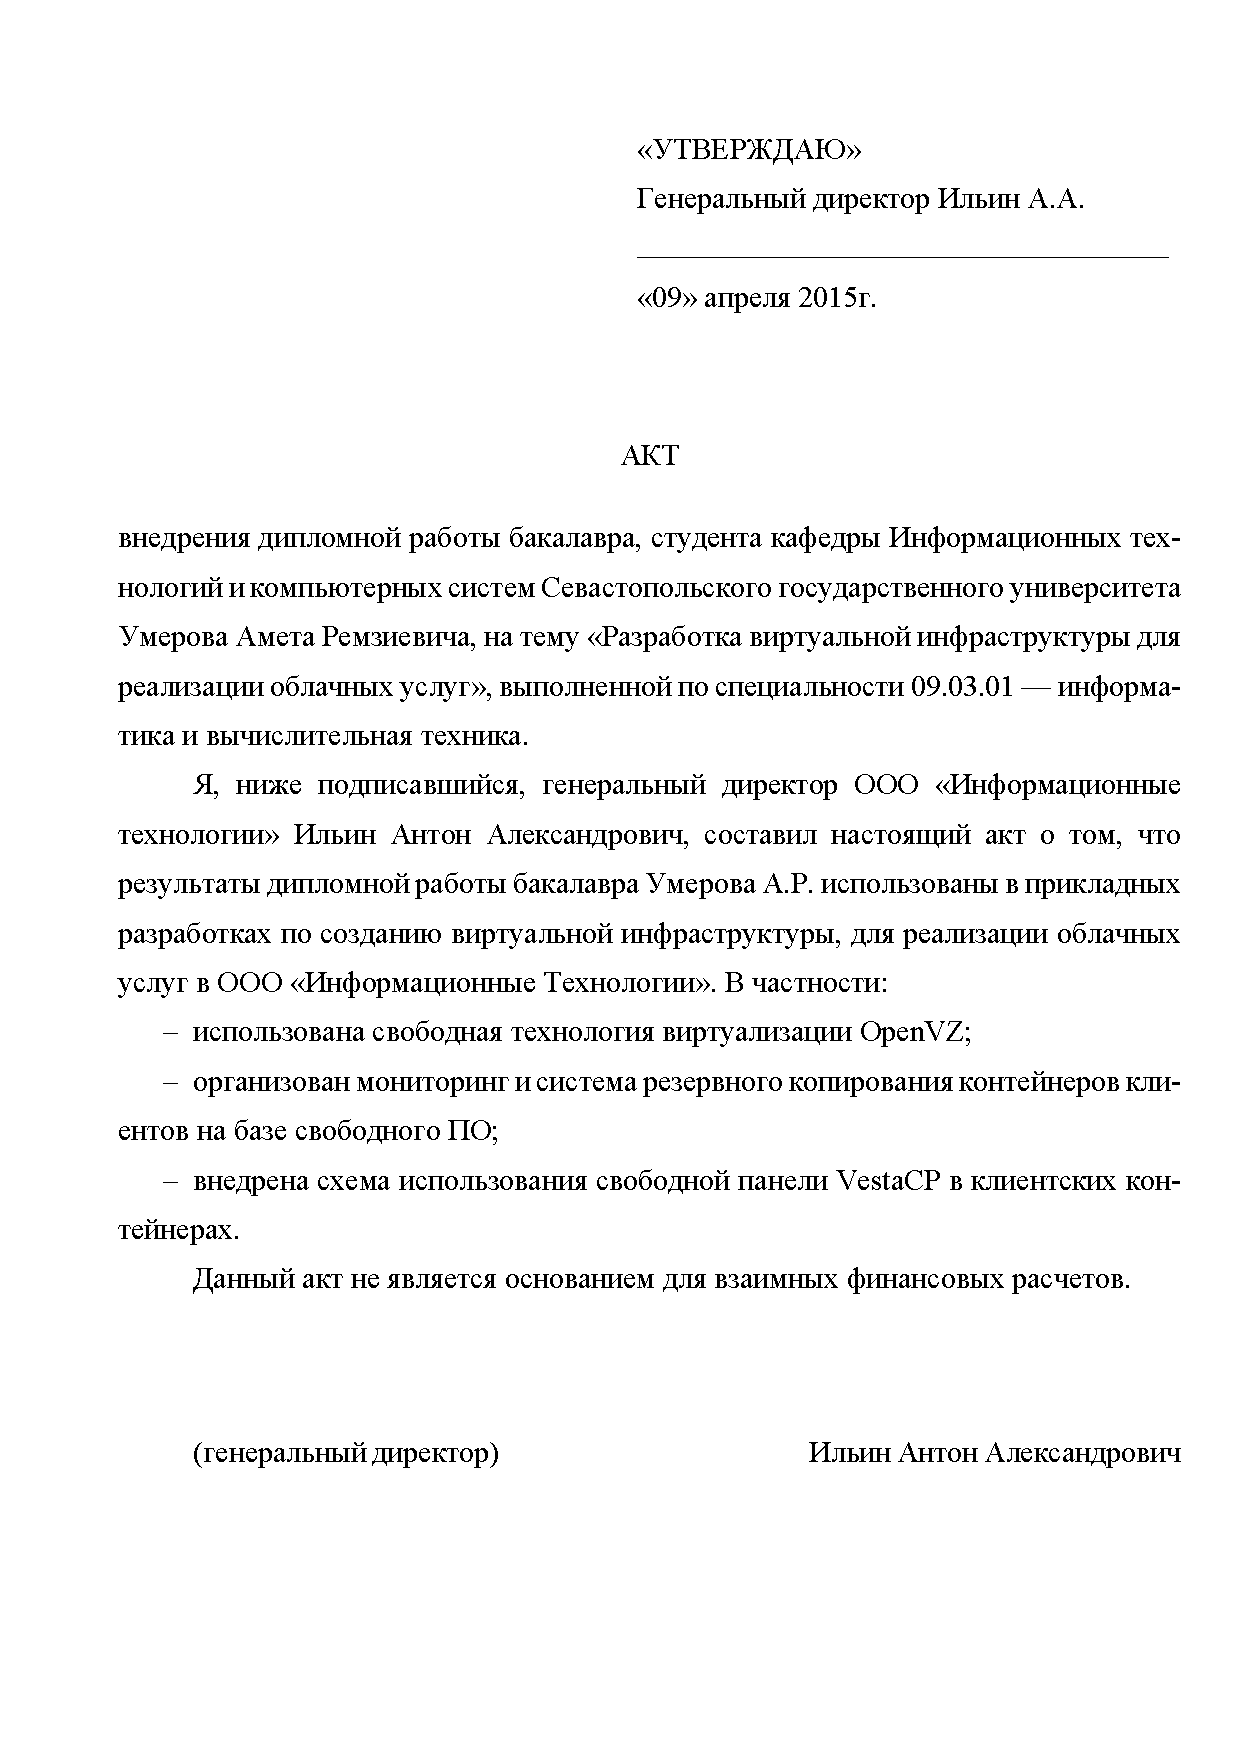
\includepdf{act} % Акт внедрения

\end{document}
%%% Конец документа
